\documentclass{standalone}
\usepackage{tikz}
\usepackage{pgfplots}
\usetikzlibrary{arrows.meta}

\begin{document}

\resizebox{8cm}{8cm}{%
    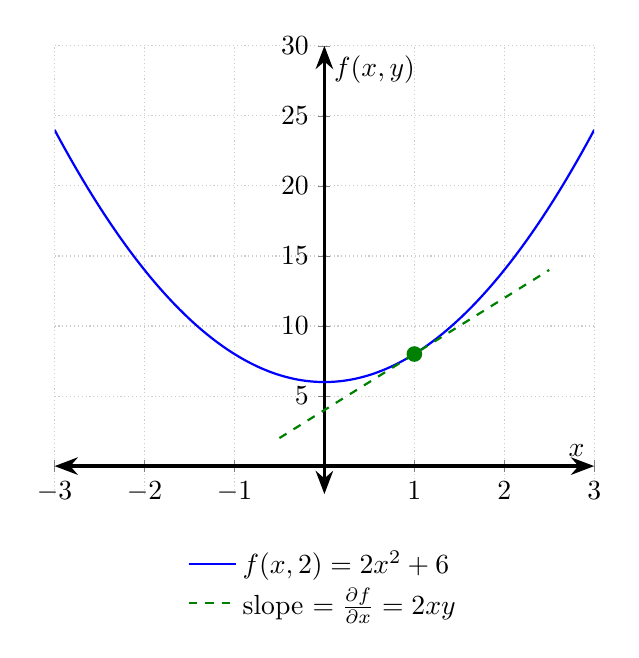
\begin{tikzpicture}
    \begin{axis}[
        title={},
        axis lines=middle,
        axis line style={Stealth-Stealth,very thick},
        xlabel=$x$,
        ylabel={$f(x, y)$},
        xmin=-3,xmax=3,ymin=-2,ymax=30,
        xtick distance=1,
        ytick distance=5,
        grid=major,
        grid style={thin,densely dotted,black!20},
        % Numbers on axes
        xtick={-3,-2,-1,0,1,2,3},
        ytick={0,5,10,15,20,25,30},
        % Legend
        legend style={
            at={(0.5,-0.1)}, % Position at the center bottom
            anchor=north, % Anchor the legend at the top
            cells={anchor=west}, % Align the legend entries to the left
            draw=none % No box around legend
        }
    ]

    % Plot the curve: f(x, 2) = 2x^2 + 6
        \addplot[
        domain=-3:3,
        samples=200,
        color=blue,
        thick
        ]
        {2*x^2 + 6};
    \addlegendentry{$f(x, 2) = 2x^2 + 6$}

    % Tangent line at x = 1: slope = 4, point (1, 8)
    % y = 8 + 4(x - 1) = 4x + 4
    \addplot[
        domain=-0.5:2.5,
        samples=2,
        color=green!50!black,
        thick,
        dashed
        ]
        {4*x + 4};
    \addlegendentry{slope $= \frac{\partial f}{\partial x} = 2xy$}

    % Mark the point at (1, 8)
    \node[circle, fill=green!50!black, inner sep=2pt] at (axis cs:1,8) {};

    \end{axis}
    \end{tikzpicture}
}

\end{document}